%%%% SEITENRAENDER, SCHRIFTGROESSE UND ZEILENABSTAND NICHT ABAENDERN => SONST GIBT ES PUNKTEABZUG
\documentclass[a4paper,11pt,singlespacing]{article}
% \usepackage[left=2.5cm,right=2.5cm,top=2.5cm]{geometry}
\usepackage{setspace}
\usepackage[utf8]{inputenc}
\usepackage[T1]{fontenc}
\usepackage{graphicx}
\usepackage[ngerman]{babel}
\usepackage{color}
\usepackage{wrapfig}
\usepackage{titleref}
\usepackage{hyperref}
\usepackage[rightcaption]{sidecap}
\usepackage{listings,xcolor}
\usepackage[numbers,round]{natbib}

% Configuration
\sloppy
\setlength{\parindent}{0ex} % Absatzeinrückung verhindern
\graphicspath{ {images/} }

\begin{document}
\pagenumbering{roman}

% Cover
\title{Systemadministration - Mailserver Honypot zum analysieren von Spam}
\author{Manuel Adams 27470, Michael Ruf 27428, Mario Waizenegger 29608}
\maketitle
\begin{abstract}
Heutzutage wird viel Spam verschickt. Einiges davon wird erkannt und gefiltert.
Das Projekt befasst sich zum einen mit der Aufgabe Spam zu erhalten und soll zum anderen als Verteiler für Spammails zu dienen.
Damit soll das Verhalten der Spammer und Spam Nachrichten analysiert werden.
\\\\
Zur Durchführung wird hierzu ein Spam Honeypot aufgesetzt.
Um die nötigen Daten zu erhalten wird der Mail-Server als Ausgangsserver offen publiziert und sich mit mehreren E-Mail-Adressen bei unsicheren Diensten registriert.
\end{abstract}

\newpage

% Table of contents
\tableofcontents

\newpage
\pagenumbering{arabic}

% Content
\section{Einleitung/Motivation}\label{sec:Einleitung}

	\subsection{Ziel der Arbeit}\label{sec:EinleitungZiel}
		Es sollen durch einen Mailserver Honeypot Erkenntnisse über Herkunft, Zweck und Zielgruppe von Spam Nachrichten erhalten werden.
		Durch diese Informationen soll die Motivation von Spammern besser verstanden und entsprechende Vorkehrungen zum Schutz erzielt werden können.
		% TODO Bisschen kurz

	\subsection{Motivation}\label{sec:EinleitungMotivation}
		Die Nachvollziehbarkeit für das Versenden vom Spam ist vielen Menschen ein Rätsel.
		Dies wirft die Fragen auf wieso jemand Spam verschicken sollte, wer Spam verschickt und warum.
		Was passiert wenn man auf Spam absichtlich reagiert?
		Ein Spam Honeypot bietet die Möglichkeit diese Fragen zu analysieren und die Daten zu erheben.
		Die Einrichtung, das Publizieren unter Spammern und der Erhalt vieler Spam Mails in kurzer Zeit ist eine gute Herausforderung.
		% - Wirtschaftlichkeit
		% - Andere Beweggründe
		% - Findet man Informationen über Systeme, von denen Spam verschickt wird?
		% - Werden die Nachrichten generiert? (Bots)
	
	\subsection{Vorgehensweise}\label{sec:EinleitungVorgehensweise}
		Eingangsserver
		\begin{enumerate}
		\item Mail Eingangsserver bereitstellen und konfigurieren
		\item DNS Server einrichten um realistische E-Mail-Adressen bereitzustellen
		\item Bei möglichst vielen Diensten mit unterschiedlichen Mailadressen registrieren
		\item Mails analysieren
		\end{enumerate}

		Ausgangsserver ("`Open Relay"') % TODO Ref Michi
		\begin{enumerate}
		\item Mail Ausgangsserver bereitstellen und konfigurieren
		\item Als "`\nameref{itm:OpenRelay}"' im Internet durchsickern lassen
		\item Eingehende Mails tatsächlich weiterleiten
		\item Mails analysieren
		\end{enumerate}

	\subsection{Aufbau der Arbeit}\label{sec:EinleitungAufbau}
		Die Hochschule Weingarten stellt für das Projekt eine \nameref{itm:VirtuelleMaschine} zur Verfügung.
		Auf dieser werden die Dienste in (virtualisierten) Containern aufgesetzt. % TODO Ref Container Manu
		Die VM muss aus Sicherheitsgründen ins interne Netz abgeschottet sein.
		Nach Außen soll der Mail-Dienst zur Nutzung als Honeypot verfügbar sein.

		Das Bild \ref{fig:Hierarchy} beschreibt den Aufbau.

		\begin{figure}
		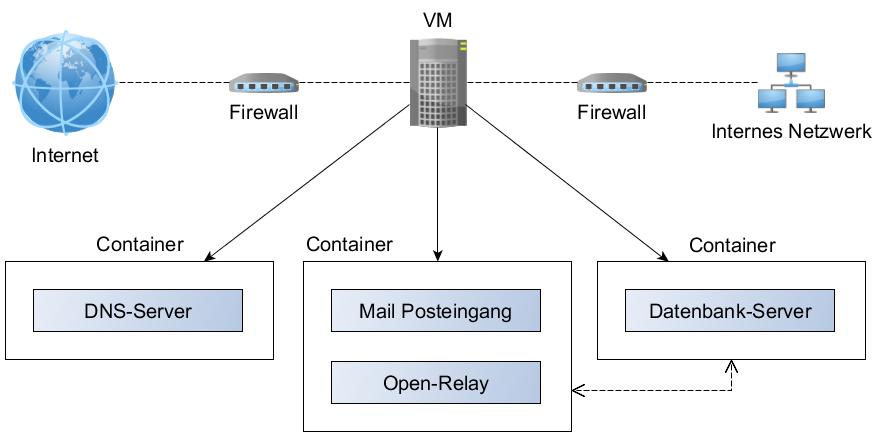
\includegraphics[width=\linewidth]{2-Hierarchy.png}
		\caption{Projektstruktur}
		\label{fig:Hierarchy}
		\end{figure}


\section{Grundbegriffe}\label{sec:Grundbegriffe}
	Die folgenden Begriffsdefinitionen und Unterscheidungen sind zum einen zur Verdeutlichung, wie Begriffe in dieser Arbeit verstanden werden und um Fachbegriffe zu erklären.
	
	\begin{description}
	\item[Honeypot\label{itm:Honeypot}]\hfill \\
		Sicherheitstechnisch scheinbar verwundbares Computerprogramm, das Computerviren, -würmer und Trojaner anlockt, um sie zu registrieren und unschädlich zu machen.\cite{Honeypot}
	\item[Open relay\label{itm:OpenRelay}]\hfill \\
		Ein SMTP-Relay-Server der durch unzureichende Sicherheitskonfiguration auch Mails weiterleitet bei denen er weder für die Absender- noch für die Zieladresse zuständig ist, wird als "`Open relay"' bezeichnet.\cite{SMTP-Relay-Server}
	\item[Virtuelle Maschine (VM)\label{itm:VirtuelleMaschine}]\hfill \\
		Eine VM ist eine Kapselung eines Rechnersystems auf Softwareebene. Dadurch lässt sich eine Rechnerarchitektur in einem Container simulieren. \cite{VM}
	\item[Blacklist \label{itm:Blacklist}]\hfill \\
		 Eine Blacklist oder "`schwarze Liste"' enthält eine Auflistung von Daten, die von einem Prozess ausgeschlossen werden solle. Das Gegenteil dazu ist eine Whitelist. \cite{Blacklist}
	% TODO Container
	\end{description}


\section{Problemstellung}\label{sec:Problemstellung}
	\subsection{Konfiguration}\label{sec:ProblemstellungKonfiguration}
		Um einen reibungslosen Ablauf zu gewährleisten muss der Mailserver in der Lage sein Mails zu empfangen und zu senden.
		Die Authentizität des Mailservers gegenüber anderen wird über verschiedene Mechanismen wie bspw. DKIM DNS-Einträge validiert. % Ref Michi
		\\
		Der Server soll als \nameref{itm:OpenRelay} dienen.
		Dabei soll der Server durch unzureichende Sicherheitskonfiguration den Versand von externen Mails erlauben.
		\\
		Mails die empfangen und gesendet werden sollen persistiert werden um jederzeit in der Lage zu sein diese Daten zu analysieren.
		Hierfür bietet sich ein Datenbank Server an. Um die Mails abzugreifen können Hooks eingesetzt werden. % Ref Michi
		Die Daten auf dem Mail-Server dürfen dadurch jederzeit verworfen werden.
		% TODO Refs and Defs

	\subsection{Mail-Adressen verteilen}\label{sec:ProblemstellungMailsVerteilen}
		Die Schwierigkeit E-Mail-Adressen als echt wirken zu lassen um damit Spam zu erhalten lässt sich durch eine frühe Verteilung bzw. Verwendung der E-Mail-Adressen bewirken.
		Daher sollen mehrere Catch-All-Mail-Adressen (TODO Def) verwendet werden um sich bei unsichere Diensten anzumelden. % Michi
		\\
		Um die E-Mail-Adresse als echt wirken zu lassen und den Erhalt zu beschleunigen bietet es sich an auf Links eingegangener Mails zu reagieren und diese anzuklicken, da Tracking-Links (TODO Def) enthalten sein können.
		\\
		Die Durchführung sollte nicht so wirken als wäre dies maschinell bzw. absichtlich.
		% TODO Refs and Defs
	
	\subsection{Open-Relay Publizieren}\label{sec:ProblemstellungPublizieren}
		Der Ausgangsserver soll als "`\nameref{itm:OpenRelay}"'" Server für Spammer dienen.
		Aufgrund dessen können versendete Spam-Mails abgehört und analyisiert werden.
		Der Honeypot muss dafür bei Spammern als unsicherer Relay-Server und guter Spamverteiler bekannt werden. % Manu
		Im Internet muss die Adresse des Servers hierzu an den richtigen Stellen verteilt werden.
		Dieser Vorgang könnte Monate dauern, daher muss noch eine Möglichkeit gefunden werden, diesen Prozess zu beschleunigen.
		\\
		Nach Möglichkeit sollte der Server nicht in einer \nameref{itm:OpenRelay} \nameref{itm:Blacklist} auftauchen, da er ansonsten nicht mehr attraktiv für Spammer ist.
		Da der Mailserver für ausschließlich Spam-Mails verwendet wird, wird sich dies wahrscheinlich nicht verhindern lassen.
		% TODO Refs and Defs

	\subsection{Analysieren}\label{sec:ProblemstellungAnalysieren}
		Da die Spam-Mails analysiert werden sollen besteht das Hauptproblem darin herauszufinden was genau Analysiert werden soll und kann.
		Falls möglich wäre es sinnvoll festzustellen ob man über Spam-Mails eventuell Informationen über das System von dem verschickt wurde erhalten kann.
		Könnte man den Weg den die Spam-Mails vom Versender bis zum Empfänger gekommen sind zurückverfolgen?
		Inwiefern lässt sich der Inhalt der Mail auf Schreibweise, Textinhalt oder auch Anhänge analysieren.
		% TODO Refs and Defs


\section{Anforderungsanalyse/Priorisierung}\label{sec:AnforderungsanalysePriorisierung}
	\begin{enumerate}
	% Michi alle items
	\item Der Mail-Server MUSS die Mails empfangen und senden können. (\autoref{sec:ProblemstellungKonfiguration})
	\item E-Mail-Adressen MÜSSEN bei diversen Diensten benutzt werden um den Erhalt von Spam einzuleiten. (\autoref{sec:ProblemstellungMailsVerteilen})
	\item Der Mail-Server SOLL bei Spammern bekannt werden. Die Honeypot Funktionalität KANN den Spammern möglichst lange unerkannt bleiben und nach Möglichkeit auf keiner "`\nameref{itm:OpenRelay}"'"~\nameref{itm:Blacklist} auftauchen. (\autoref{sec:ProblemstellungPublizieren})
	\item Die E-Mails MÜSSEN analysiert werden können. (\autoref{sec:ProblemstellungAnalysieren})
	\end{enumerate}


%\section{Lösungsvorschläge}\label{sec:Lösungsvorschläge}
%	TODO
%
%
%\section{Auswahl Lösung anhand Anforderungen}\label{sec:AuswahlLösungAnhandAnforderungen}
%	TODO
%
%
%\section{Umsetzung}\label{sec:Umsetzung}
%	TODO
%
%
%\section{Fazit/Ausblick/Übertragbarkeit}\label{sec:Fazit/Ausblick/Übertragbarkeit}
%	TODO


\newpage

% Quotes
\bibliography{zitate}
\bibliographystyle{plain}
\addcontentsline{toc}{section}{Literatur}

% Image listing
\listoffigures
\addcontentsline{toc}{section}{Abbildungsverzeichnis}

% Listings (code examples, ...)
\lstlistoflistings
\addcontentsline{toc}{section}{Listings}

\newpage

% Additional stuff
\section*{Anhang}\label{Anhang}
\addcontentsline{toc}{section}{Anhang}

%\newpage
%
%% Plagiarism declaration
%\section*{Eidesstattliche Erklärung}\label{sec:Eidesstattliche Erklärung}

\end{document}